\newpage

\section{Архитектура объединённой сети фирмы}

\subsection{Общая схема сети}

Объединенная сеть состоит из сети центрального офиса, сети 1 филиала и сети 2 филиала. Её общая схема изображена на рисунке~\ref{pic:3_1}. В графических обозначениях схема изображена на рисунке~\ref{pic:3_2}.

\begin{figure}[h]
\center{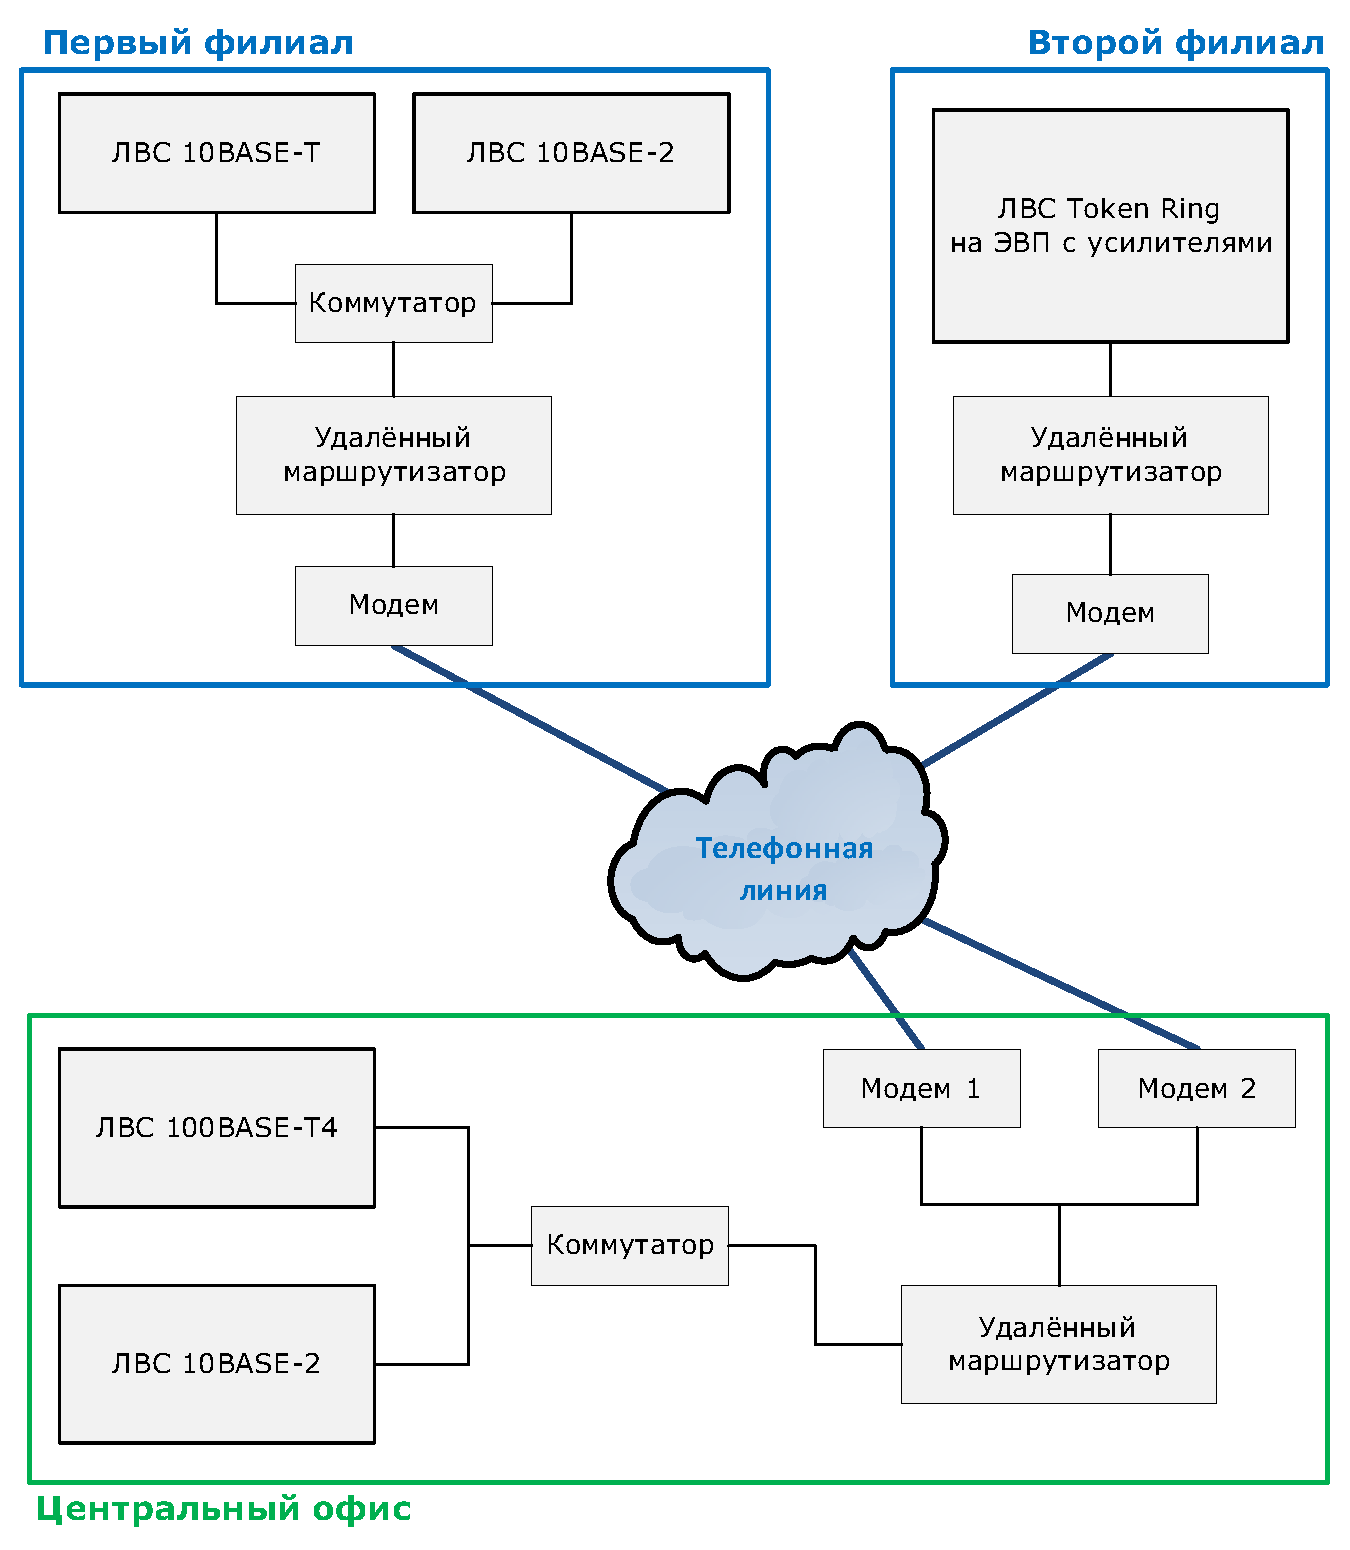
\includegraphics[width=0.6\linewidth]{pics/pic3_1.eps}}
\caption{Общая схема РСОД фирмы.}
\label{pic:3_1}
\end{figure}

В центральном офисе фирмы расположены ЛВС 100BASE-T4 и ЛВС 10BASE-2. Обе сети подключены к коммутатору, к которому также подключён удаленный маршрутизатор с двумя модемами.\par\bigskip

В первом филиале фирмы расположены ЛВС 10BASE-T и ЛВС 10BASE-2. Обе сети подключены к коммутатору, к нему также подключен удаленный маршрутизатор с одним модемом.\par\bigskip

\newpage

Во втором филиале фирмы расположена ЛВС Token Ring на STP c усилителями.

\begin{figure}[h]
\center{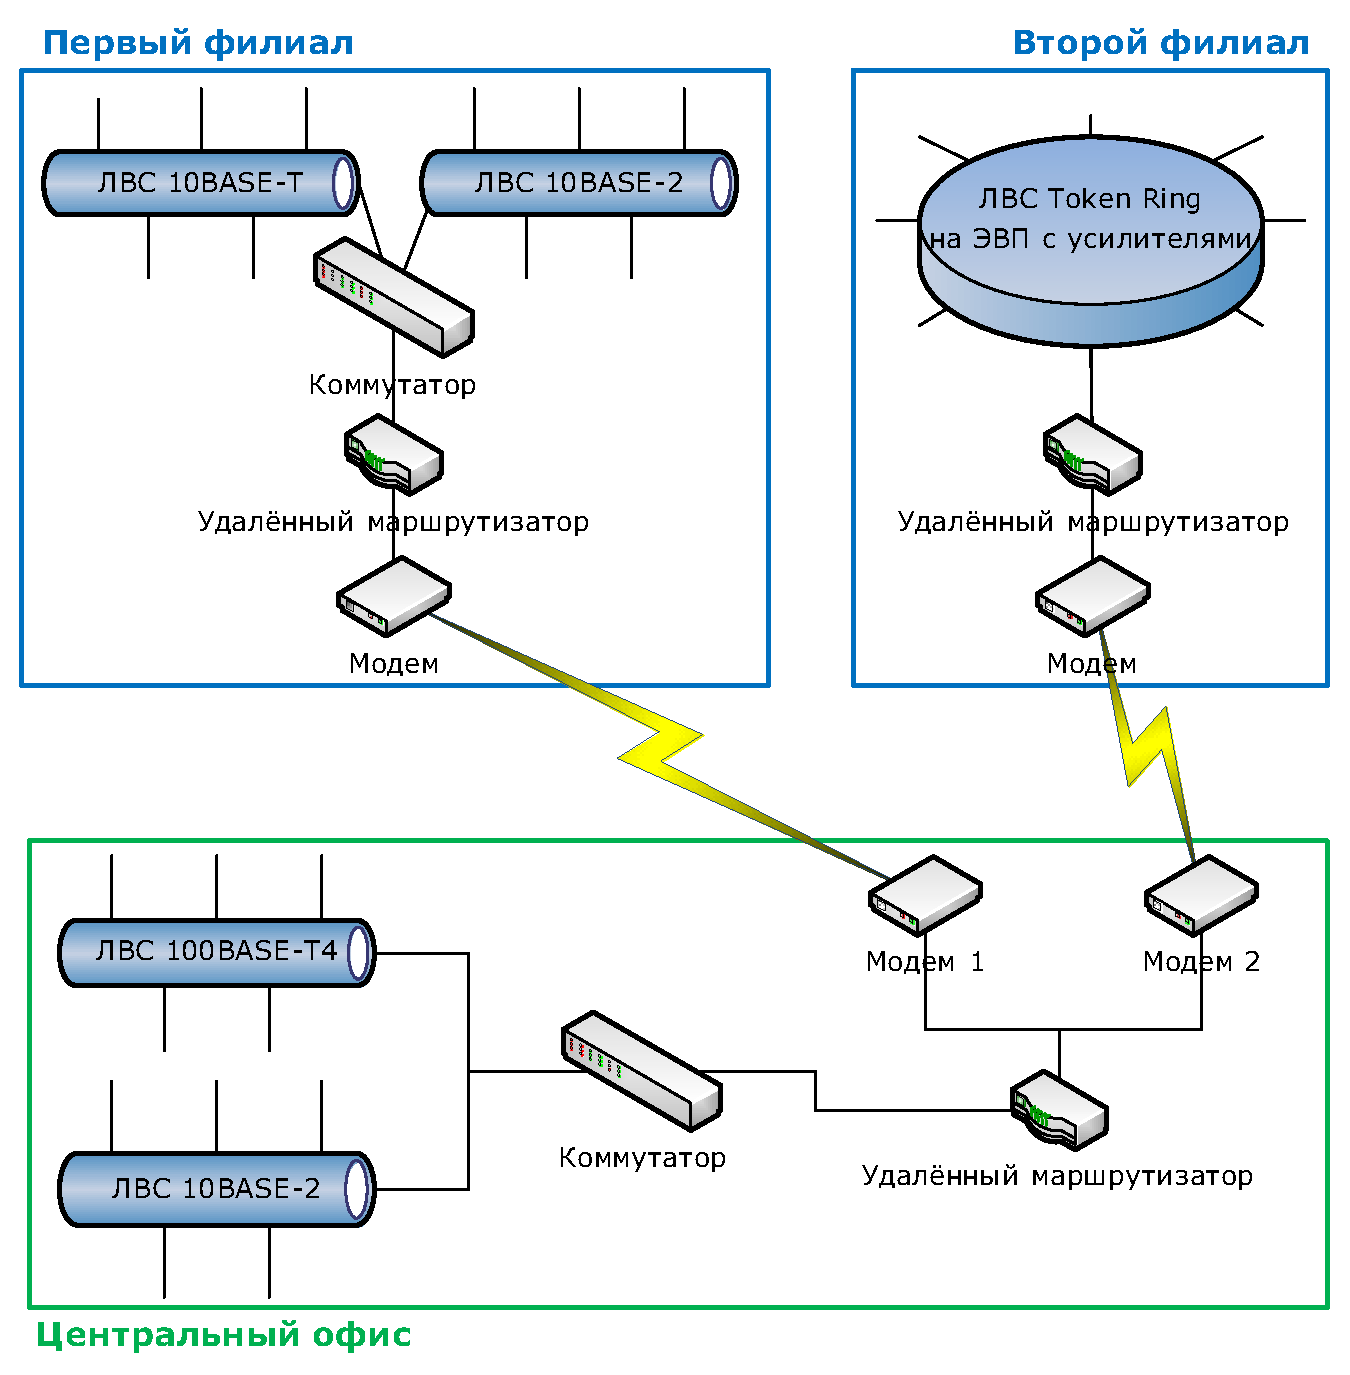
\includegraphics[width=0.6\linewidth]{pics/pic3_2.eps}}
\caption{Общая схема РСОД фирмы в графических обозначениях.}
\label{pic:3_2}
\end{figure}

\newpage

\subsection{Схема сети центрального офиса}

В центральном офисе фирмы расположены ЛВС 100BASE-T4, содержащая 2 концентратора, и ЛВС 10BASE-2, содержащая 2 сегмента. Обе сети подключены к коммутатору, к которому также подключён удаленный маршрутизатор с двумя модемами. В офисе также находится сервер фирмы. Схема сети представлена на рисунке~\ref{pic:3_3}.

\begin{figure}[h]
\center{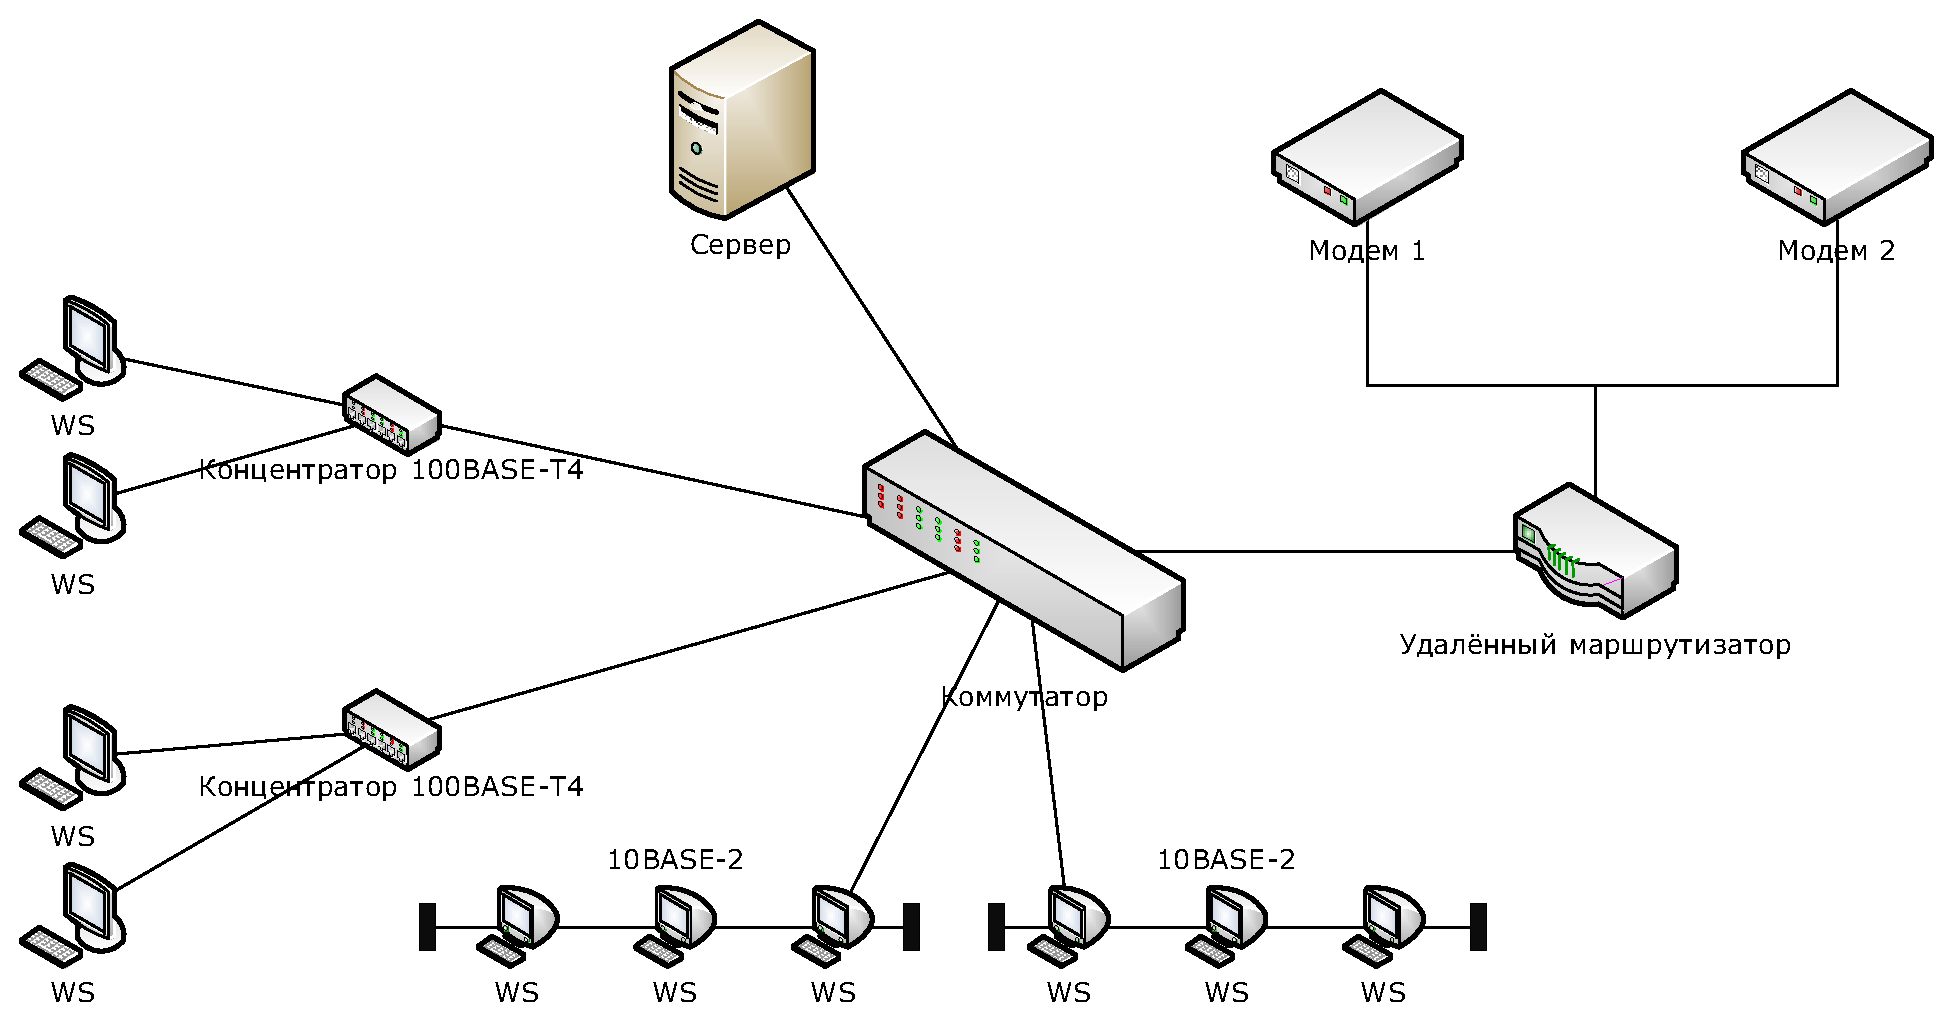
\includegraphics[width=0.6\linewidth]{pics/pic3_3.eps}}
\caption{Схема сети центрального офиса.}
\label{pic:3_3}
\end{figure}

\newpage

\subsection{Схема сети первого филиала}

В первом филиале фирмы расположены ЛВС 10BASE-T, содержащая 4 концентратора, и ЛВС 10BASE-2, содержащая 4 сегмента. Обе сети подключены к коммутатору, к нему также подключен удаленный маршрутизатор с одним модемом. Схема сети представлена на рисунке~\ref{pic:3_4}.

\begin{figure}[h]
\center{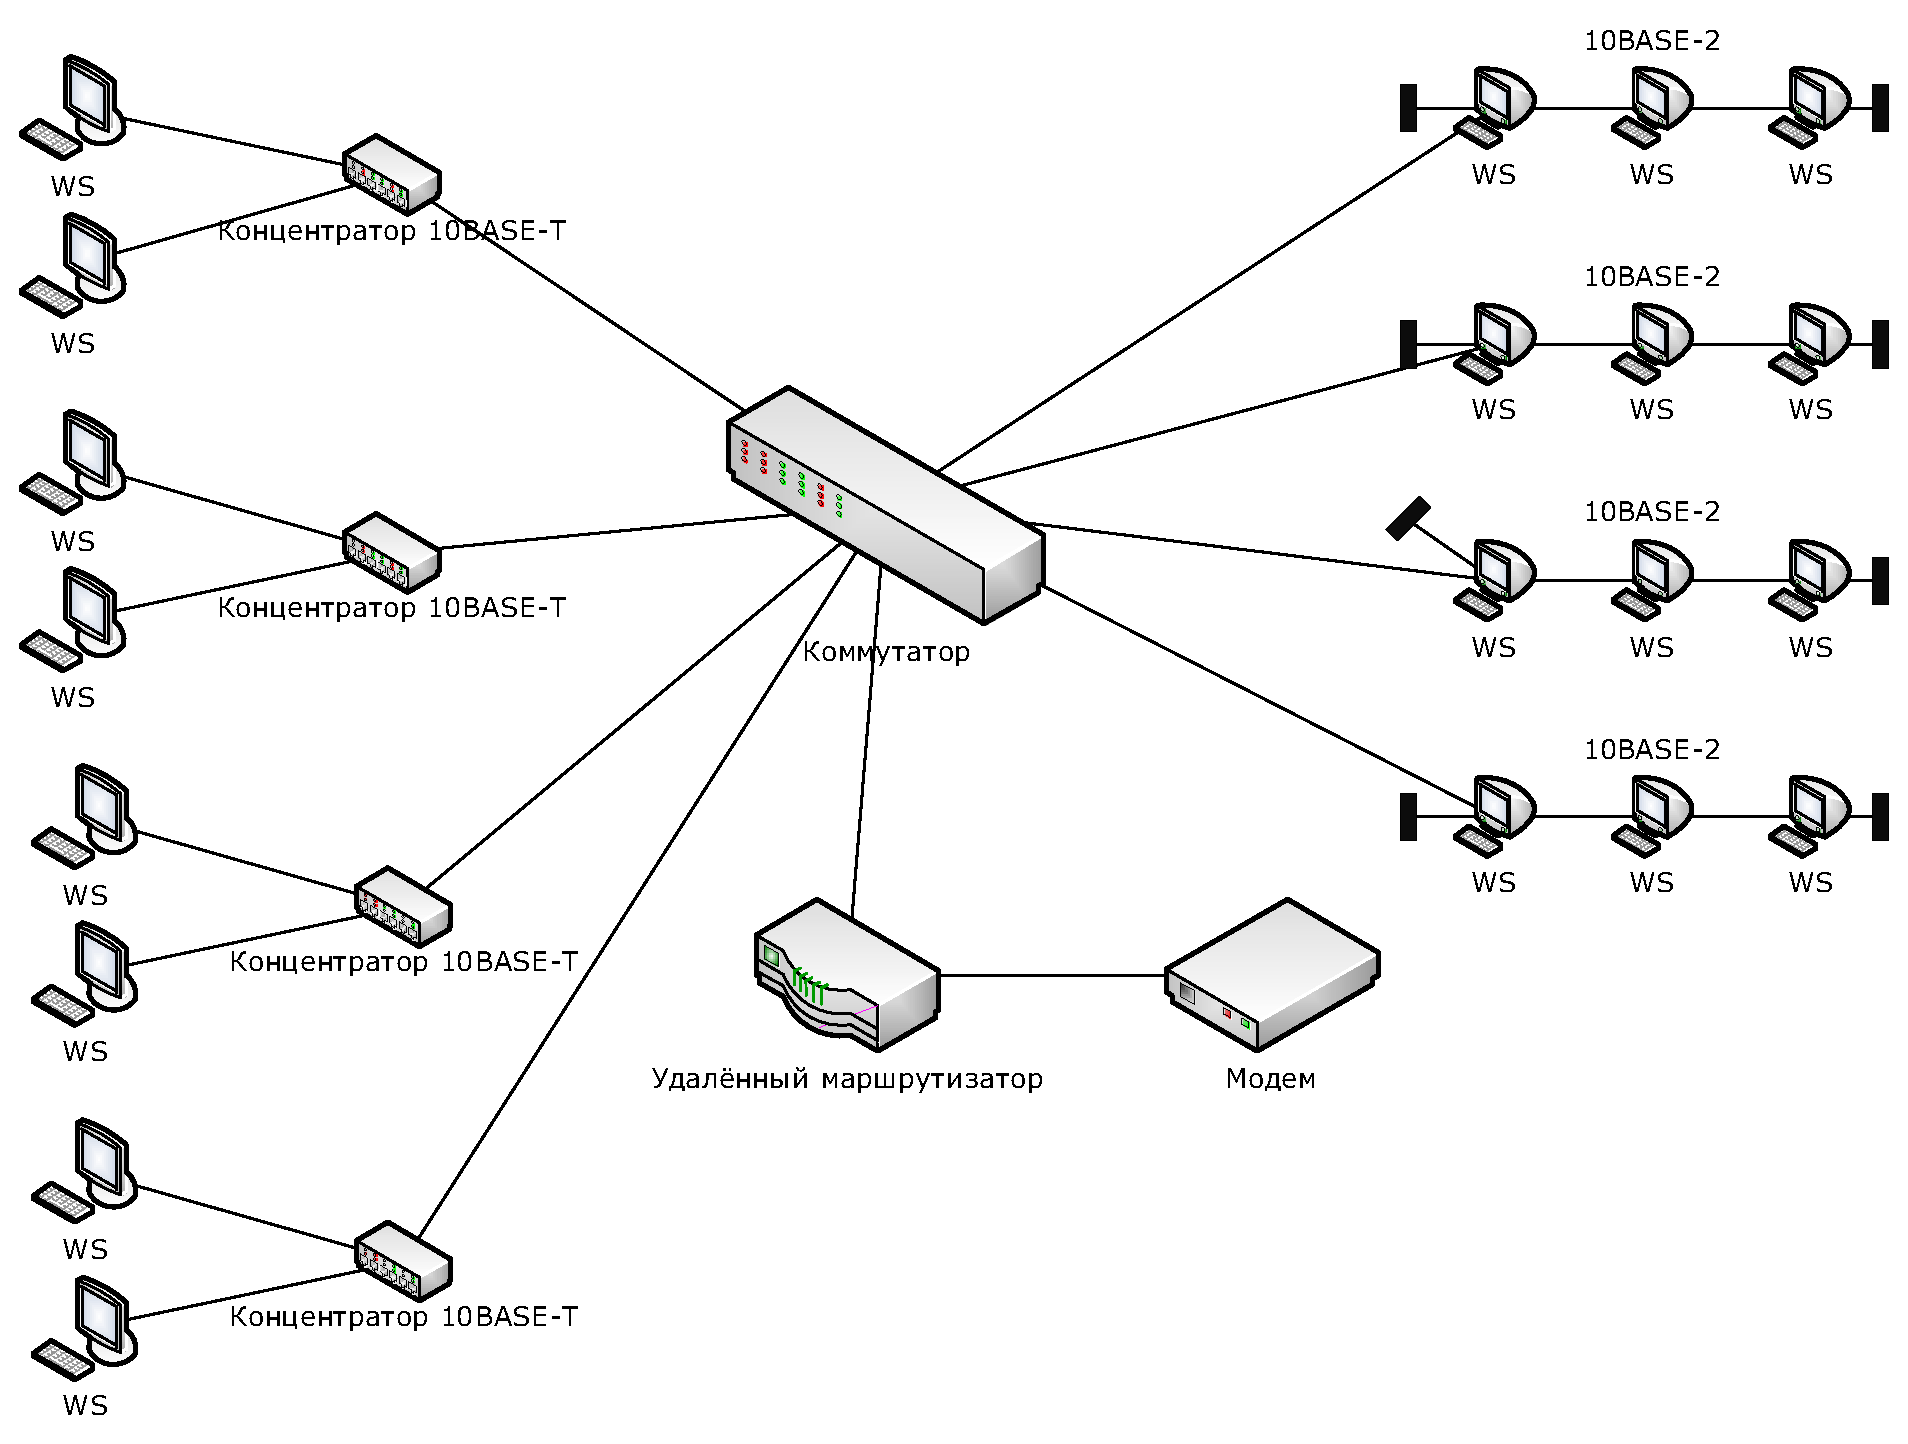
\includegraphics[width=0.6\linewidth]{pics/pic3_4.eps}}
\caption{Схема сети первого филиала.}
\label{pic:3_4}
\end{figure}

\newpage

\subsection{Схема сети второго филиала}

Во втором филиале фирмы расположена ЛВС Token Ring на STP с усилителями. Схема сети представлена на рисунке~\ref{pic:3_5}.

\begin{figure}[h]
\center{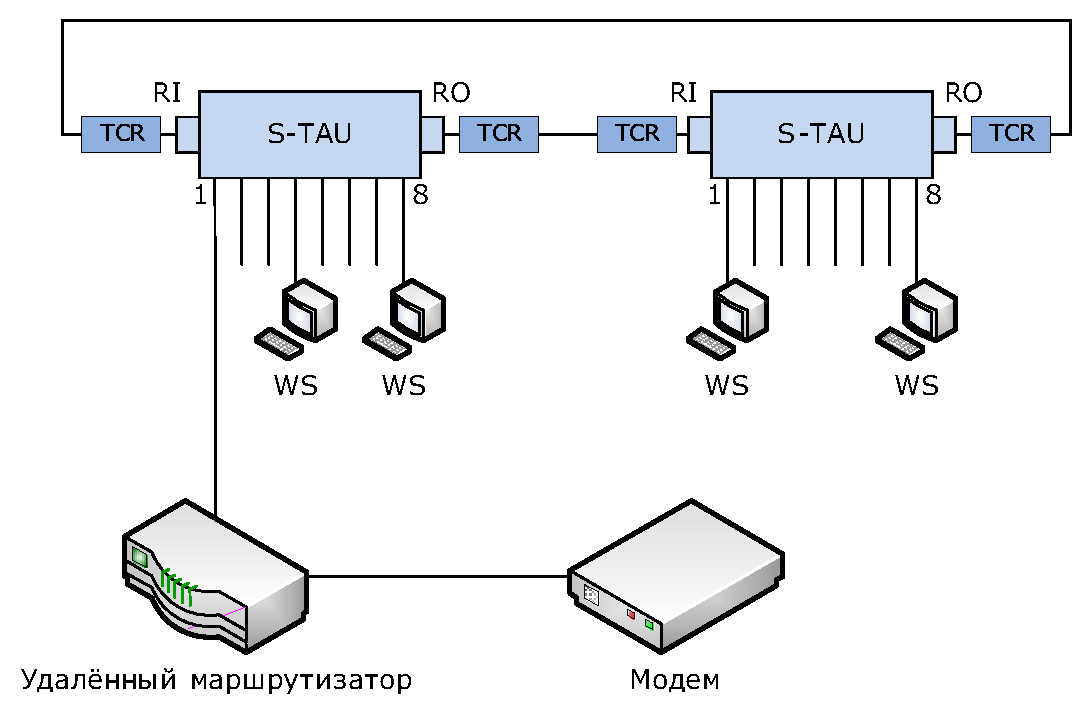
\includegraphics[width=0.6\linewidth]{pics/pic3_5.eps}}
\caption{Схема сети второго филиала.}
\label{pic:3_5}
\end{figure}

\newpage

\subsection{Правила построения сети}

Для построения работоспособной сети следует придерживаться ряда правил.

\subsubsection{Правила построения сетей 100BASE-T4}

При построении сети на основе 100BASE-T4 применяются следующие правила:
\begin{itemize}
\item для перехода с технологии TX на T4 требуется заменить концентраторы и сетевые адаптеры, тогда не придётся менять километры кабеля, так как кабель используется тот же;
\item в кабеле используются все 4 пары;
\item длина луча сети должна быть не более 100 метров;
\item между любыми двумя узлами сети расстояние должно быть не более 205 м;
\item между любыми двумя узлами должно быть не более 5 сегментов и 4 повторителей;
\end{itemize}

\subsubsection{Правила построения сетей 10BASE-2}

При построении сети на основе 10Base2 применяются следующие правила:
\begin{itemize}
\item используется тонкий коаксиальный кабель с терминаторами на обоих концах;
\item для усиления сигнала используются повторители;
\item повторители должны быть подключены к источнику электропитания;
\item рабочие станции подключаются к кабелю с помощью сетевых адаптеров с разъёмом BNC и T-коннекторов;
\item один из терминаторов каждого сегмента заземляется;
\item T-коннектор подключается к терминатору непосредственно или через расстояние кратное 2.5 м;
\item минимальное расстояние между двумя Т-коннекторами составляет 2.5 м;
\item расстояние между двумя Т-коннекторами должно быть кратно 2.5 м;
\item между любыми двумя узлами должно находиться не более 5 сегментов, 4 повторителей;
\item длина сегмента не более 185 м;
\item длина сети не более 925 м;
\item к сегменту может быть подключено не более 30 узлов.
\end{itemize}

\subsubsection{Правила построения сетей 10BASE-T}

При построении сети на основе 10Base2 применяются следующие правила:
\begin{itemize}
\item длина сегмента – 100 метров;
\item между двумя узлами может быть не выше 5 лучей; 
\item общее количество станций не должно превышать 1024;
\item максимальное число концентраторов между любыми двумя станциями сети - 4;
\item мксимальный диаметр сети - 500 м;
\item используются коннекторы RJ-45;
\item не допускается образование колец;
\item используется неэкранированная витая пара 3 категории.
\end{itemize}

\subsubsection{Правила построения сетей Token Ring}

При построении сети на основе Token Ring STP применяются следующие правила:
\begin{itemize}
\item в качестве кабеля используется экранированная витая пара (STP);
\item для доступа с сети используются S-TAU (не более 12 штук);
\item максимум в сети может быть 255 узлов;
\item применяются усилители на медном кабеле (TCR), расстояние между устройствами доступа составляет 300 м;
\item максимальная длина луча без усилителя составляет 100 м.
\end{itemize}
